\newpage
\section{SAR polarimetry applications}\label{sec:polarimetry}
%add intro
This section describes how to use the applications related to SAR polarimetry.

\subsection{Matrices conversions}\label{ssec:polconv}

This applications allows converting classical polarimetric matrices to each other.
For instance, it is possible to get the coherency matrix from the Sinclar one, or the Mueller matrix from the coherency one.
The figure below (\ref{fig:polconv}) shows the workflow used in this application.

\begin{figure}[h]
  \centering
   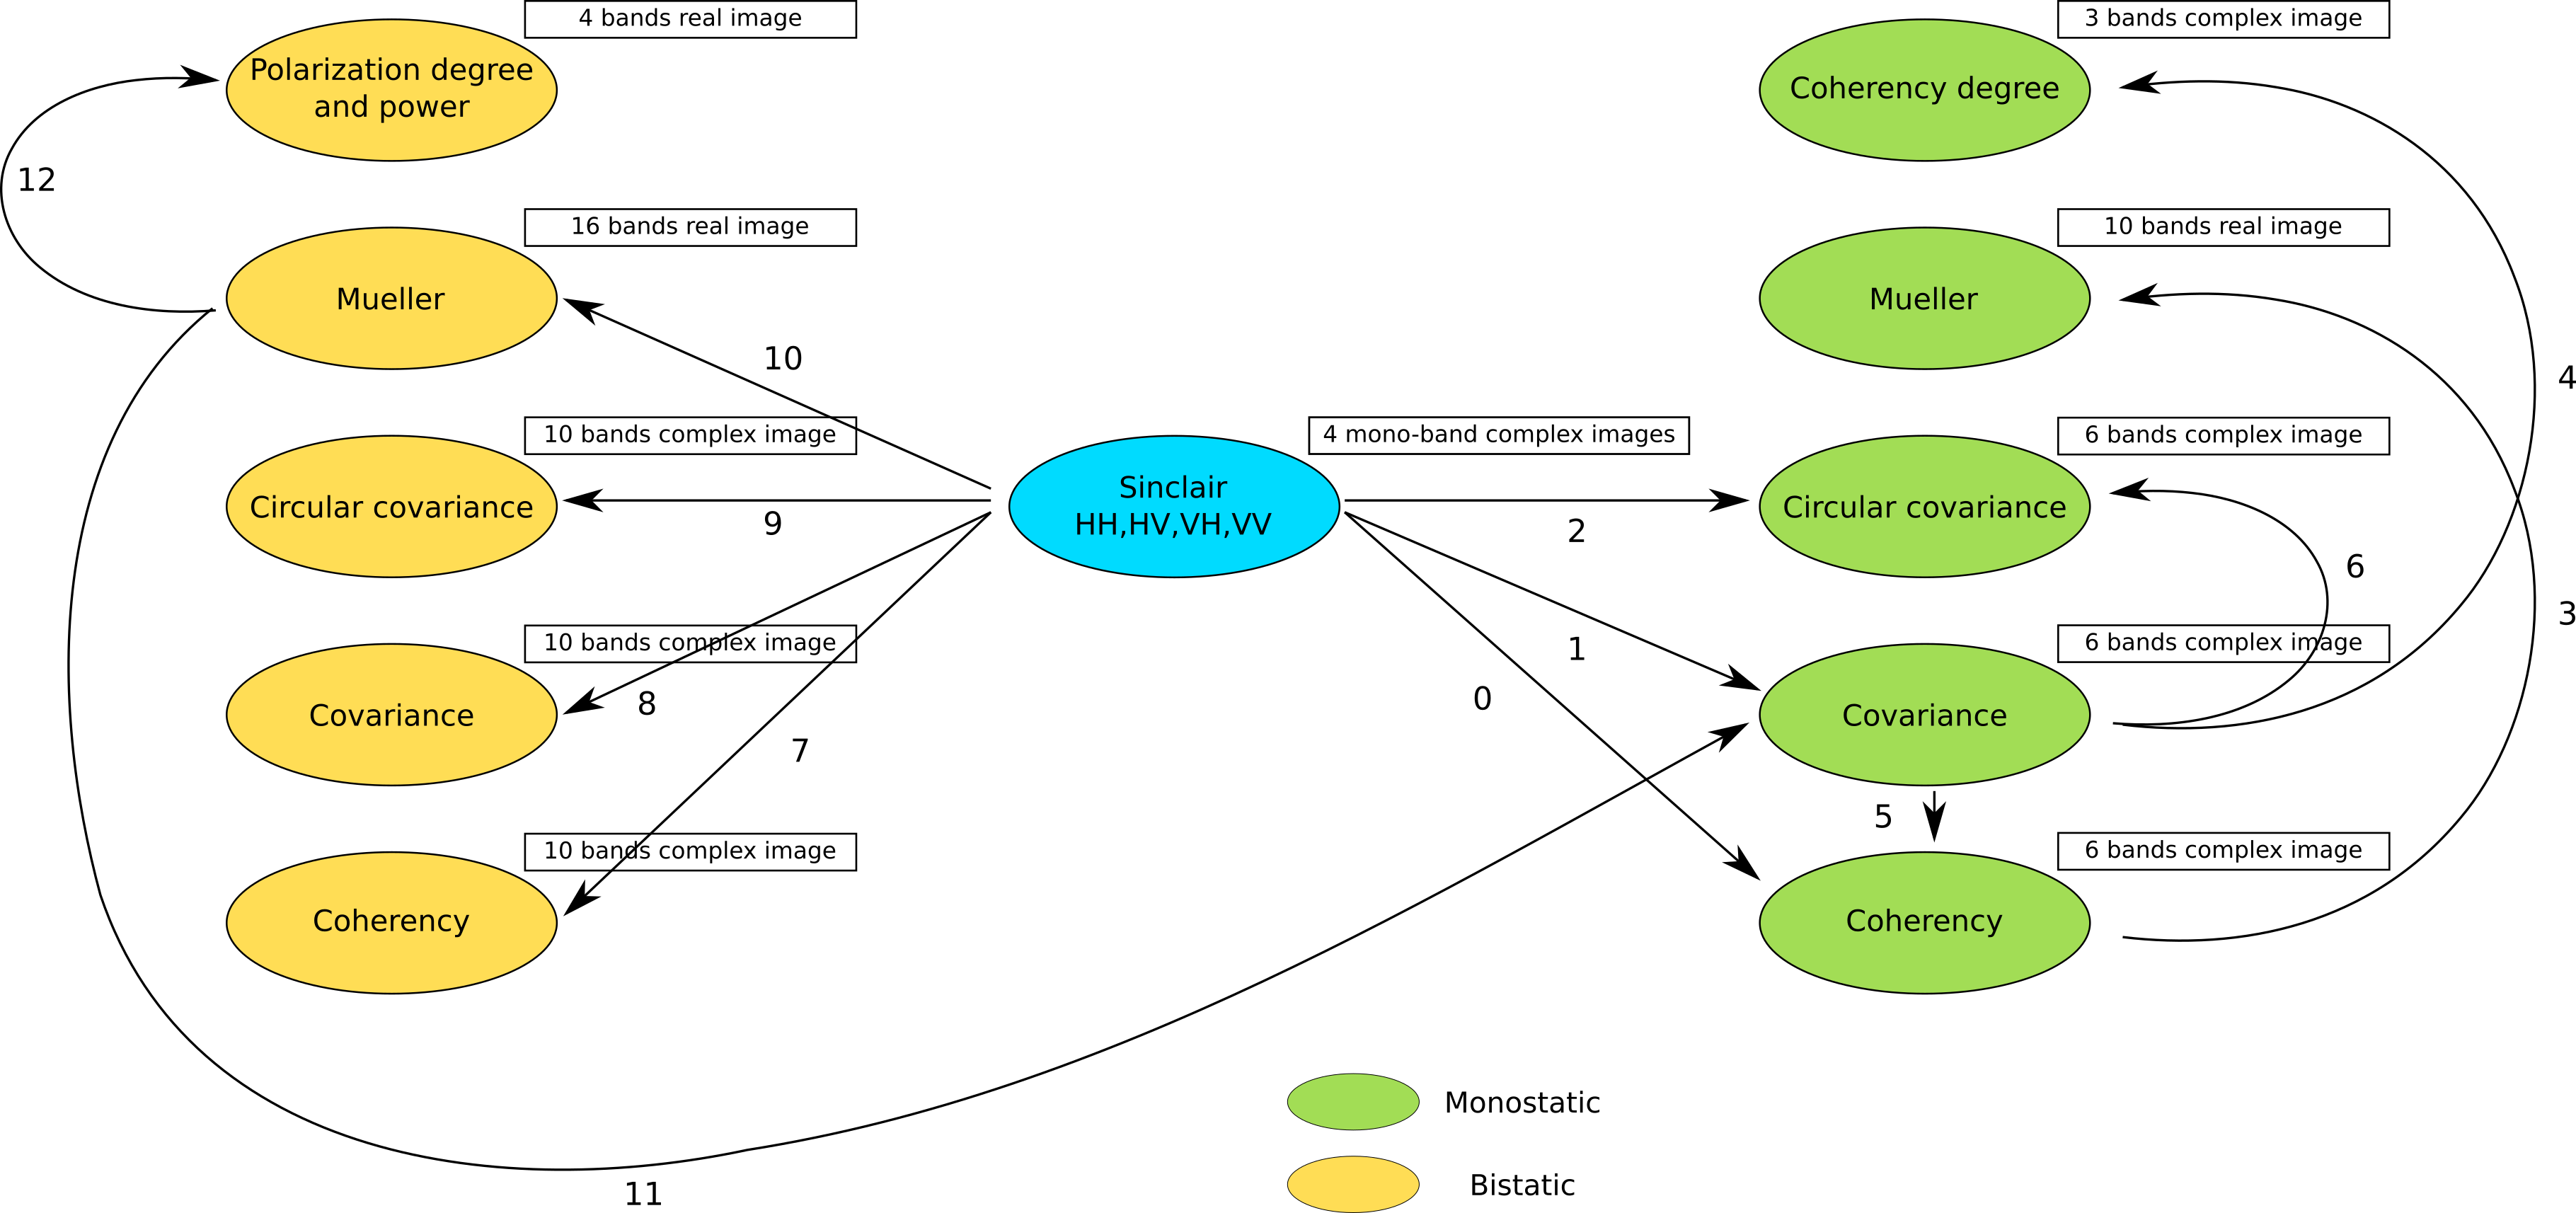
\includegraphics[width=\textwidth]{../Art/sarpol_conversion_schema.png}
  \itkcaption[SAR polarimetry conversion]{SAR polarimetry conversion application.}
  \label{fig:polconv}
\end{figure}

The filters used in this application never handle matrices, but images where each band is related to their elements.
As most of the time SAR polarimetry handles symetric matrices, only the relevant elements are stored, so that the images representing them have a minimal number of bands.
For instance, the coherency matrix size is 3x3 in the monostatic case, and 4x4 in the bistatic case : it will thus be stored in a 6-band or a 10-band complex image (the diagonal and the upper elements of the matrix).

The Sinclair matrix is a special case : it is always represented as 3 or 4 one-band complex images (for mono- or bistatic case).

There are 13 available conversions, each one being related to the following  parameters: \newline
    0. msinclairtocoherency \newline
    1. msinclairtocovariance \newline
    2. msinclairtocircovariance \newline
    3. mcoherencytomueller \newline
    4. mcovariancetocoherencydegree \newline
    5. mcovariancetocoherency \newline
    6. mlinearcovariancetocircularcovariance \newline
    7. bsinclairtocoherency \newline
    8. bsinclairtocovariance \newline
    9. bsinclairtocircovariance \newline
    10. bsinclairtomueller \newline
    11. bmuellertomcovariance \newline
    12. bmuellertopoldegandpower \newline
    


For each option parameter, the list below gives the formula used.

--- Monostatic case ---   \newline
    
0. msinclairtocoherency (SinclairToReciprocalCoherencyMatrixFunctor) \newline
- channel #0 : \f$ (S_{hh}+S_{vv}).(S_{hh}+S_{vv})^{*} \f$ \newline
- channel #1 : \f$ (S_{hh}+S_{vv}).(S_{hh}-S_{vv})^{*} \f$ \newline
- channel #2 : \f$ (S_{hh}+S_{vv}).(2*S_{hv})^{*} \f$ \newline
- channel #3 : \f$ (S_{hh}-S_{vv}).(S_{hh}-S_{vv})^{*} \f$ \newline
- channel #4 : \f$ (S_{hh}-S_{vv}).(2*S_{hv})^{*} \f$ \newline
- channel #5 : \f$ (2*S_{hv}).(2*S_{hv})^{*} \f$ \newline
 
1. msinclairtocovariance (SinclairToReciprocalCovarianceMatrixFunctor) \newline
- channel #0 : \f$ S_{hh}.S_{hh}^{*} \f$ \newline
- channel #1 : \f$ S_{hh}.S_{hv}^{*} \f$ \newline
- channel #2 : \f$ S_{hh}.S_{vv}^{*} \f$ \newline
- channel #3 : \f$ S_{hv}.S_{hv}^{*} \f$ \newline
- channel #4 : \f$ S_{hv}.S_{vv}^{*} \f$ \newline
- channel #5 : \f$ S_{vv}.S_{vv}^{*} \f$ \newline
 
2. msinclairtocircovariance (SinclairToReciprocalCircularCovarianceMatrixFunctor) \newline
- channel #0 : \f$ S_{ll}.S_{ll}^{*} \f$ \newline
- channel #1 : \f$ S_{ll}.S_{lr}^{*} \f$ \newline
- channel #2 : \f$ S_{ll}.S_{rr}^{*} \f$ \newline
- channel #3 : \f$ S_{lr}.S_{lr}^{*} \f$ \newline
- channel #4 : \f$ S_{lr}.S_{rr}^{*} \f$ \newline
- channel #5 : \f$ S_{rr}.S_{rr}^{*} \f$ \newline
 
3. mcoherencytomueller (ReciprocalCoherencyToReciprocalMuellerFunctor) \newline
- channel #0 : \f$ 0.5*\mathcal{Re}( Coherency[0]+Coherency[3]+Coherency[5]) \f$ \newline
- channel #1 : \f$ 0.5*\mathcal{Re}( Coherency[0]+Coherency[3]-Coherency[5]) \f$ \newline
- channel #2 : \f$ 0.5*\mathcal{Re}( Coherency[0]-Coherency[3]+Coherency[5]) \f$ \newline
- channel #3 : \f$ 0.5*\mathcal{Re}(-Coherency[0]+Coherency[3]+Coherency[5]) \f$ \newline
- channel #4 : \f$ \mathcal{Re}(Coherency[1]) \f$ \newline
- channel #5 : \f$ \mathcal{Re}(Coherency[2]) \f$ \newline
- channel #6 : \f$ \mathcal{Im}(Coherency[4]) \f$ \newline
- channel #7 : \f$ \mathcal{Re}(Coherency[4]) \f$ \newline
- channel #8 : \f$ \mathcal{Im}(Coherency[2]) \f$ \newline
- channel #9 : \f$ \mathcal{Im}(Coherency[1]) \f$ \newline
 
4. mcovariancetocoherencydegree (ReciprocalCovarianceToCoherencyDegreeFunctor) \newline
- channel #0 : \f$ abs(S_{hh}*S_{vv}}^{*}) / sqrt(S_{hh}*S_{hh}}^{*}) / sqrt(S_{vv}*S_{vv}}^{*}) \f$ \newline
- channel #1 : \f$ abs(S_{hv}*S_{vv}}^{*}) / sqrt(S_{hv}*S_{hv}}^{*}) / sqrt(S_{vv}*S_{vv}}^{*}) \f$ \newline
- channel #2 : \f$ abs(S_{hh}*S_{hv}}^{*}) / sqrt(S_{hh}*S_{hh}}^{*}) / sqrt(S_{hv}*S_{hv}}^{*}) \f$ \newline
 
5. mcovariancetocoherency (ReciprocalCovarianceToReciprocalCoherencyFunctor) \newline
- channel #0 : \f$ 0.5(S_{hh}+S_{vv}.(S_{hh}+S_{vv})^{*} \f$ \newline
- channel #1 : \f$ 0.5(S_{hh}+S_{vv}.(S_{hh}-S_{vv})^{*} \f$ \newline
- channel #2 : \f$ (S_{hh}+S_{vv}.(S_{hv})^{*} \f$ \newline
- channel #3 : \f$ 0.5(S_{hh}-S_{vv}.(S_{hh}-S_{vv})^{*} \f$ \newline
- channel #4 : \f$ (S_{hh}-S_{vv}.(S_{hv})^{*} \f$ \newline
- channel #5 : \f$ 2.0*S_{hv}.S_{hv}^{*} \f$ \newline
 
6. mlinearcovariancetocircularcovariance (ReciprocalLinearCovarianceToReciprocalCircularCovarianceFunctor) \newline
- channel #0 : \f$ 0.25(C_{1}+C_{3}+4*C_{2}-2*C_{6}-4*C_{5}-4*C_{9}) \f$ \newline
- channel #1 : \f$ 0.25(C_{1}-C_{3}+2*C_{5}+2*C_{9} - 0.5\mathcal{i}.(C_{4}+C_{7}+C_{8}) \f$ \newline
- channel #2 : \f$ 0.25(C_{1}+C_{3}-4*C_{2}-2*C_{6} - \mathcal{i}.(C_{4}+C_{8}) \f$ \newline
- channel #3 : \f$ 0.25(C_{1}+C_{3}+2*C_{6} \f$ \newline
- channel #4 : \f$ 0.25(C_{1}-C_{3}+2*C_{5}-2*C_{9} - 0.5\mathcal{i}.(C_{4}-C_{7}+C_{8}) \f$ \newline
- channel #5 : \f$ 0.25(C_{1}+C_{3}+4*C_{2}-2*C_{6}+4*C_{5}+4*C_{9}) \f$ \newline

Where: \newline
- \f$ C_{1} = S_{hh}*S_{hh}}^{*} = \mathcal{Re}(input[0]) \f$ \newline
- \f$ C_{2} = S_{hv}*S_{hv}}^{*} = \mathcal{Re}(input[3]) \f$ \newline
- \f$ C_{3} = S_{vv}*S_{vv}}^{*} = \mathcal{Re}(input[5]) \f$ \newline
- \f$ C_{4} = \mathcal{Re}(S_{hh}*S_{hv}}^{*}) = \mathcal{Re}(input[1]) \f$ \newline
- \f$ C_{5} = \mathcal{Im}(S_{hh}*S_{hv}}^{*}) = \mathcal{Im}(input[1]) \f$ \newline
- \f$ C_{6} = \mathcal{Re}(S_{hh}*S_{vv}}^{*}) = \mathcal{Re}(input[2]) \f$ \newline
- \f$ C_{7} = \mathcal{Im}(S_{hh}*S_{vv}}^{*}) = \mathcal{Im}(input[2]) \f$ \newline
- \f$ C_{8} = \mathcal{Re}(S_{hv}*S_{vv}}^{*}) = \mathcal{Re}(input[4]) \f$ \newline
- \f$ C_{9} = \mathcal{Im}(S_{hv}*S_{vv}}^{*} = \mathcal{Im}(input[4])) \f$ \newline
 
 
--- Bistatic case --- \newline 

7. bsinclairtocoherency (SinclairToCoherencyMatrixFunctor) \newline
 - channel #0 : \f$ (S_{hh}+S_{vv}).(S_{hh}+S_{vv})^{*} \f$ \newline
 - channel #1 : \f$ (S_{hh}+S_{vv}).(S_{hh}-S_{vv})^{*} \f$ \newline
 - channel #2 : \f$ (S_{hh}+S_{vv}).(S_{hv}+S_{vh})^{*} \f$ \newline
 - channel #3 : \f$ (S_{hh}+S_{vv}).(j(S_{hv}-S_{vh}))^{*} \f$ \newline
 - channel #4 : \f$ (S_{hh}-S_{vv}).(S_{hh}-S_{vv})^{*} \f$ \newline
 - channel #5 : \f$ (S_{hh}-S_{vv}).(S_{hv}+S_{vh})^{*} \f$ \newline
 - channel #6 : \f$ (S_{hh}-S_{vv}).(j(S_{hv}-S_{vh}))^{*} \f$ \newline
 - channel #7 : \f$ (S_{hv}+S_{vh}).(S_{hv}+S_{vh})^{*} \f$ \newline
 - channel #8 : \f$ (S_{hv}+S_{vh}).(j(S_{hv}-S_{vh}))^{*} \f$ \newline
 - channel #9 : \f$ j(S_{hv}-S_{vh}).(j(S_{hv}-S_{vh}))^{*} \f$ \newline
 
8. bsinclairtocovariance (SinclairToCovarianceMatrixFunctor) \newline
- channel #0 : \f$ S_{hh}.S_{hh}^{*} \f$ \newline
- channel #1 : \f$ S_{hh}.S_{hv}^{*} \f$ \newline
- channel #2 : \f$ S_{hh}.S_{vh}^{*} \f$ \newline
- channel #3 : \f$ S_{hh}.S_{vv}^{*} \f$ \newline
- channel #4 : \f$ S_{hv}.S_{hv}^{*} \f$ \newline
- channel #5 : \f$ S_{hv}.S_{vh}^{*} \f$ \newline
- channel #6 : \f$ S_{hv}.S_{vv}^{*} \f$ \newline
- channel #7 : \f$ S_{vh}.S_{vh}^{*} \f$ \newline
- channel #8 : \f$ S_{vh}.S_{vv}^{*} \f$ \newline
- channel #9 : \f$ S_{vv}.S_{vv}^{*} \f$ \newline
 
9. bsinclairtocircovariance (SinclairToCircularCovarianceMatrixFunctor) \newline
- channel #0 : \f$ S_{ll}.S_{ll}^{*} \f$ \newline
- channel #1 : \f$ S_{ll}.S_{lr}^{*} \f$ \newline
- channel #2 : \f$ S_{ll}.S_{rl}^{*} \f$ \newline
- channel #3 : \f$ S_{ll}.S_{rr}^{*} \f$ \newline
- channel #4 : \f$ S_{lr}.S_{lr}^{*} \f$ \newline
- channel #5 : \f$ S_{lr}.S_{rl}^{*} \f$ \newline
- channel #6 : \f$ S_{lr}.S_{rr}^{*} \f$ \newline
- channel #7 : \f$ S_{rl}.S_{rl}^{*} \f$ \newline
- channel #8 : \f$ S_{rl}.S_{rr}^{*} \f$ \newline
- channel #9 : \f$ S_{rr}.S_{rr}^{*} \f$ \newline
With: \newline
- \f$ S_{ll} = 0.5(-S_{hh}-i*S_{hv}-i*S_{vh}+S_{vv}) \f$ \newline
- \f$ S_{lr} = 0.5(-S_{hh}+i*S_{hv}-i*S_{vh}+S_{vv}) \f$ \newline
- \f$ S_{rl} = 0.5(-S_{hh}-i*S_{hv}+i*S_{vh}-S_{vv}) \f$ \newline
- \f$ S_{rr} = 0.5(-S_{hh}+i*S_{hv}+i*S_{vh}+S_{vv}) \f$ \newline
 
10. bsinclairtomueller (SinclairToMueller) \newline
- channel #0  : \f$ 0.5\mathcal{Re}( T_{xx}.T_{xx}^{*} + T_{xy}.T_{xy}^{*} + T_{yx}.T_{yx}^{*} + T_{yy}.T_{yy}^{*} ) \f$ \newline
- channel #1  : \f$ 0.5\mathcal{Re}( T_{xx}.T_{xx}^{*} - T_{xy}.T_{xy}^{*} + T_{yx}.T_{yx}^{*} - T_{yy}.T_{yy}^{*} ) \f$ \newline
- channel #2  : \f$ \mathcal{Re}( T_{xx}.T_{xy}^{*} + T_{yx}.T_{yy}^{*} ) \f$ \newline
- channel #3  : \f$ \mathcal{Im}( T_{xx}.T_{xy}^{*} + T_{yx}.T_{yy}^{*} ) \f$ \newline
- channel #4  : \f$ 0.5\mathcal{Re}( T_{xx}.T_{xx}^{*} + T_{xy}.T_{xy}^{*} - T_{yx}.T_{yx}^{*} - T_{yy}.T_{yy}^{*} ) \f$ \newline
- channel #5  : \f$ 0.5\mathcal{Re}( T_{xx}.T_{xx}^{*} - T_{xy}.T_{xy}^{*} - T_{yx}.T_{yx}^{*} + T_{yy}.T_{yy}^{*} ) \f$ \newline
- channel #6  : \f$ \mathcal{Re}( T_{xx}.T_{xy}^{*} - T_{yx}.T_{yy}^{*} ) \f$ \newline
- channel #7  : \f$ \mathcal{Im}( T_{xx}.T_{xy}^{*} - T_{yx}.T_{yy}^{*} ) \f$ \newline
- channel #8  : \f$ \mathcal{Re}( T_{xx}.T_{yx}^{*} + T_{xy}.T_{yy}^{*} ) \f$ \newline
- channel #9  : \f$ \mathcal{Im}( T_{xx}.T_{yx}^{*} - T_{xy}.T_{yy}^{*} ) \f$ \newline
- channel #10 : \f$ \mathcal{Re}( T_{xx}.T_{yy}^{*} + T_{xy}.T_{yx}^{*} ) \f$ \newline
- channel #11 : \f$ \mathcal{Im}( T_{xx}.T_{yy}^{*} - T_{xy}.T_{yx}^{*} ) \f$ \newline
- channel #12 : \f$ \mathcal{Re}( T_{xx}.T_{yx}^{*} + T_{xy}.T_{yy}^{*} ) \f$ \newline
- channel #13 : \f$ \mathcal{Im}( T_{xx}.T_{yx}^{*} - T_{xy}.T_{yy}^{*} ) \f$ \newline
- channel #14 : \f$ \mathcal{Re}( T_{xx}.T_{yy}^{*} + T_{xy}.T_{yx}^{*} ) \f$ \newline
- channel #15 : \f$ \mathcal{Im}( T_{xx}.T_{yy}^{*} - T_{xy}.T_{yx}^{*} ) \f$ \newline

With :\newline
- \f$ T_{xx} = -S_{hh} \f$ \newline
- \f$ T_{xy} = -S_{hv} \f$ \newline
- \f$ T_{yx} = -S_{vh} \f$ \newline
- \f$ T_{yy} = -S_{vv} \f$ \newline
 
 
11. bmuellertomcovariance (MuellerToReciprocalCovarianceFunctor) \newline
- channel #0 : \f$ 0.5*(M_{11} + M_{22} + 2*M_{12}) \f$ \newline
- channel #1 : \f$ 0.5*(M_{11} - M_{22}) \f$ \newline
- channel #2 : \f$ 0.5*(M_{11} + M_{22} - 2*M_{12}) \f$ \newline
- channel #3 : \f$ 0.5*(M_{13} + M_{23} + i*(M_{14}+M_{24})) \f$ \newline
- channel #4 : \f$ 0.5*(M_{33} - M_{44} - 2*i*M_{34}) \f$ \newline
- channel #5 : \f$ 0.5*(M_{13} - M_{23} - i*(M_{14}-M_{24})) \f$ \newline
 
12. bmuellertopoldegandpower (MuellerToPolarisationDegreeAndPowerFunctor) \newline
- channel #0 : \f$ P_{min} \f$ \newline
- channel #1 : \f$ P_{max} \f$ \newline
- channel #2 : \f$ DegP_{min} \f$ \newline
- channel #3 : \f$ DegP_{max} \f$ \newline


\subsection{Polarimetric decompositions}\label{ssec:poldecomp}

From one-band complex images (HH, HV, VH, VV), returns the selected decomposition.
The H-alpha-A decomposition is currently the only one available; it is implemented for the monostatic case (transmitter and receiver are co-located).
User must provide three one-band complex images HH, HV or VH, and VV (HV = VH in monostatic case).
The applications returns a float vector image, made of three channels : H (entropy), Alpha, A (Anisotropy).

In order to do so, the complex coherency matrix (size 3*3) must be diagonalized.
The H-alpha-A decomposition thus uses the following filters : SinclairToReciprocalCoherencyMatrixFunctor and ReciprocalHAlphaImageFilter.
Here are the formula used (refer to the previous section about how the covariance matrix is obtained from the sinclair one):

- channel #0 : \f$ entropy = -\sum_{i=0}^{2}{p[i].\log{p[i]}} / \log{3} \f$ \newline
- channel #1 : \f$ \alpha = \sum_{i=0}^{2}{p[i].\alpha_{i} \f$ \newline
- channel #2 : \f$ anisotropy = \frac {SortedEigenValues[1] - SortedEigenValues[2]}{SortedEigenValues[1] + SortedEigenValues[2]} \f$ \newline

Where: \newline
- \f$ p[i] = max(SortedEigenValues[i], 0) / \sum_{i=0}^{2, SortedEigenValues[i]>0}{SortedEigenValues[i]} \f$ \newline
- \f$ \alpha_{i} = \left| SortedEigenVector[i] \right|* \frac{180}{\pi}\f$ \newline

With: \newline
- \f$ if p[i] < 0, p[i]=0 \f$ \newline
- \f$ if p[i] > 1, p[i]=1 \f$ \newline
- \f$ if \alpha_{i} > 90, \alpha_{i}=90 \f$ \newline

\subsection{Polarimetric synthetis}\label{ssec:polsynth}

This application gives, for each pixel, the power that would have been received by a SAR system with a basis different from the classical (H,V) one (polarimetric synthetis). 
The new basis are indicated through two Jones vectors, defined by the user thanks to orientation (psi) and ellipticity (khi) parameters.
These parameters are namely psii, khii, psir and khir. The suffixes (i) and (r) refer to the transmiting antenna and the receiving antenna respectively.
Orientations and ellipticities are given in degrees, and are between -90/90 degrees and -45/45 degrees respectively.\n " 

Four polarization architectures can be processed : \newline
1) HH\_HV\_VH\_VV : full polarization, general bistatic case. \newline
2) HH\_HV\_VV or HH\_VH\_VV : full polarization, monostatic case (transmitter and receiver are co-located). \newline
3) HH\_HV : dual polarization. \newline
4) VH\_VV : dual polarization. \newline
The application takes a complex vector image as input, where each band correspond to a particular emission/reception polarization scheme.
User must comply with the band order given above, since the bands are used to build the Sinclair matrix.

In order to determine the architecture, the application first relies on the number of bands of the input image. \newline
1) Architecture HH\_HV\_VH\_VV is the only one with four bands, there is no possible confusion. \newline
2) Concerning HH\_HV\_VV and HH\_VH\_VV architectures, both correspond to a three channels image. But they are processed in the same way, as the Sinclair matrix is symetric in the monostatic case. \newline
3) Finally, the two last architectures (dual polarizations), can't be distinguished only by the number of bands of the input image. User must then use the parameters emissionh and emissionv to indicate the architecture of the system : emissionh=1 and emissionv=0 for HH\_HV,  emissionh=0 and emissionv=1 for VH\_VV. \newline
Note : if the architecture is HH\_HV, khii and psii are automatically set to 0/0 degrees; if the architecture is VH\_VV, khii and psii are automatically set to 0/90 degrees.

It is also possible to force the calculation to co-polar or cross-polar modes.
In the co-polar case, values for psir and khir will be ignored and forced to psii and khii; same as the cross-polar mode, where khir and psir will be forced to psii + 90 degrees and -khii.

Finally, the result of the polarimetric synthetis is expressed in the power domain, through a one-band scalar image. \newline
Note: this application doesn't take into account the terms which do not depend on the polarization of the antennas. 
The parameter gain can be used for this purpose. \newline

 
The final formula is thus : \begin{verbatim} P = gain x | B^T . [S] . A |^2 \end{verbatim}, where A ans B are two Jones vectors and S is a Sinclair matrix."

 \newline
 
The two figures below (\ref{fig:polsynthll} and \ref{fig:polsynthlr}) show the two images obtained with the basis LL and LR (L for left circular polarization and R for right polarization),
from a Radarsat 2 image taken over Vancouver. Once the four two-band images imagery\_HH imagery\_HV imagery\_VH imagery\_VV were merged 
into a single four complex band image imageryC\_HH\_HV\_VH\_VV.tif, the following commands were used to produce the LL and LR images :

\begin{verbatim} otbcli_SARPolarSynth -in imageryC_HH_HV_VH_VV.tif 
									  -psii 0 -khii 45 -mode co -out test-LL.tif \end{verbatim}
\begin{verbatim} otbcli_SARPolarSynth -in imageryC_HH_HV_VH_VV.tif 
									  -psii 0 -khii 45 -mode cross -out test-LR.tif \end{verbatim}

The produced images were then rescaled to intensities ranging from 0 to 255 in order to be displayed.

\begin{figure}
  \centering
  \begin{subfigure}
   \centering
    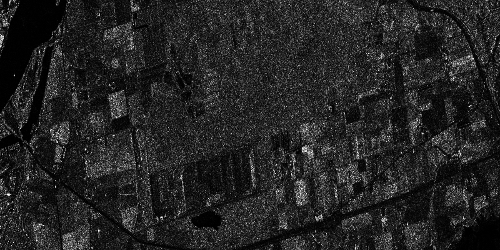
\includegraphics[width=\textwidth]{../Art/test-left-co-2.png}
    \itkcaption[SAR polarimetry conversion]{Image LL}
    \label{fig:polsynthll}
   \end{subfigure}
   
   \begin{subfigure}
   \centering
    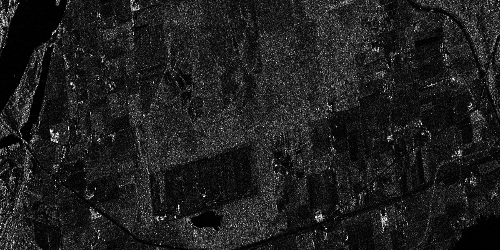
\includegraphics[width=\textwidth]{../Art/test-left-cross-2.png}
    \itkcaption[SAR polarimetry conversion]{Image LR}
    \label{fig:polsynthll}
   \end{subfigure}
\end{figure}
